\begin{table}[h!]
\centering
\renewcommand{\arraystretch}{1.4}
\resizebox{\textwidth}{!}{%
\begin{tabular}{lllll}
\toprule
\textbf{Cell} & \textbf{Firing Rate (Hz)} & \textbf{Reference} & \textbf{Sparsity} & \textbf{Reference} \\
\midrule


\multirow{6}{*}{$\vcenter{\hbox{
\includegraphics[height=1.5em]{figures/neurons/mgc.png}}}$ Mature granule}
  & 1.2 (0.56--2.38)                        & \textcite{mchughAdultborn2022}
  & 2--5\%                                  & \textcite{galloniRecurrent2022, hainmuellerParallel2018} \\
  & 0.49                                    & \textcite{diamantakiSparse2016}
  & 9\%                                     & \textcite{goodsmithSpatial2017} \\
  & $0.031 \pm 0.096$                       & \textcite{zhangSelective2020}
  & & \\
  & 0.4                                     & \textcite{wheelerHippocampomeorg2023}
  & & \\
  & $0.96 \pm 0.19$                         & \textcite{goodsmithDentate2019}
  & & \\
  & $\approx 0.2$                           & \textcite{senzaiExtracellular2016}
  & & \\
  & $72 \pm 8$\textsuperscript{max}         & \textcite{lubkeSpecialized1998}
  & & \\
\midrule


$\vcenter{\hbox{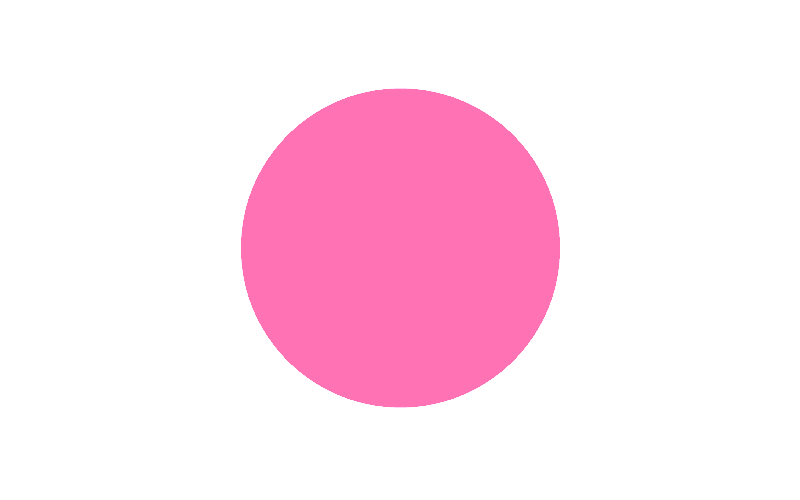
\includegraphics[height=1.5em]{figures/neurons/igc.png}}}$ Immature granule
  & 2.3 (1.6--6.7)                         & \textcite{mchughAdultborn2022}
  & & \\
\midrule


\multirow{3}{*}{$\vcenter{\hbox{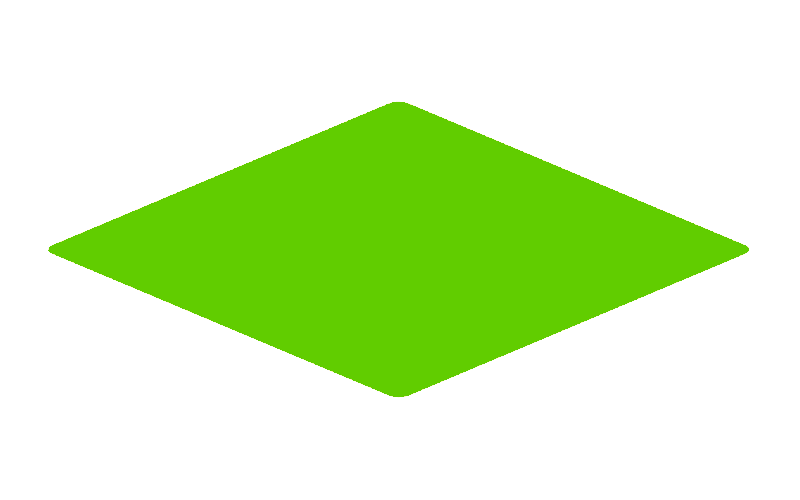
\includegraphics[height=1.5em]{figures/neurons/mc.png}}}$ Mossy}
  & 0.84                                    & \textcite{wheelerHippocampomeorg2023}
  & $\approx 100\%$                         & \textcite{danielsonVivo2017} \\
  & $1.05 \pm 0.07$                         & \textcite{goodsmithDentate2019}
  & 88\%                                    & \textcite{goodsmithSpatial2017} \\
  & $\approx 0.8$                           & \textcite{senzaiExtracellular2016}
  & & \\
  & $50 \pm 6$\textsuperscript{max}         & \textcite{lubkeSpecialized1998}
  & & \\
\midrule

$\vcenter{\hbox{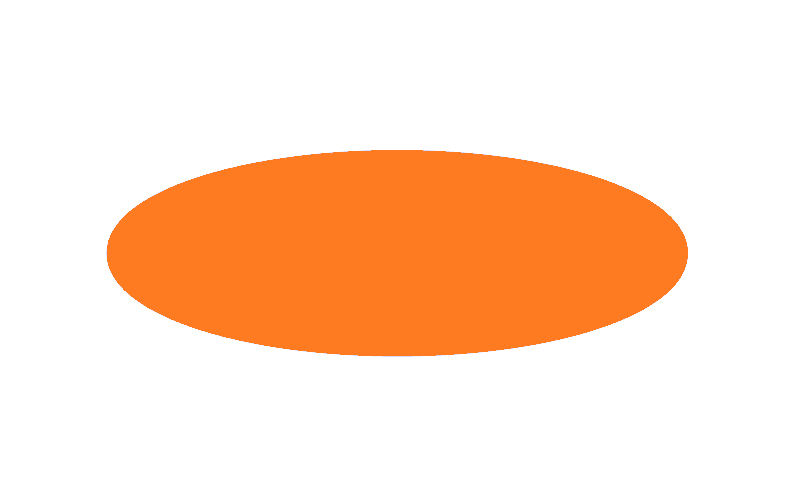
\includegraphics[height=1.5em]{figures/neurons/hipp.png}}}$ HIPP
  & ---                                     &
  & & \\
\midrule

\multirow{2}{*}{$\vcenter{\hbox{
\includegraphics[height=1.5em]{figures/neurons/bc.png}}}$ Basket}
  & $13.6 \pm 0.8$                          & \textcite{liSustained2022}
  & & \\
  & $230 \pm 15$\textsuperscript{max}       & \textcite{lubkeSpecialized1998}
  & & \\
\midrule


\multirow{7}{*}{$\vcenter{\hbox{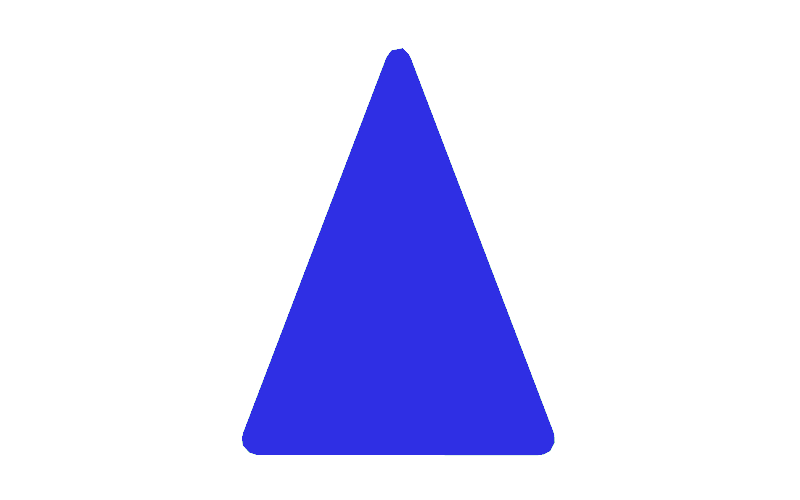
\includegraphics[height=1.5em]{figures/neurons/pca3.png}}}$ CA3 pyramidal}
  & 0.2                                     & \textcite{mizusekiPreconfigured2013}
  & 29\%                                    & \textcite{goodsmithSpatial2017} \\
  & 0.5                                     & \textcite{kayHippocampal2016}
  & 20--30\%                                & \textcite{galloniRecurrent2022} \\
  & $0.72 \pm 0.51$                         & \textcite{lasztocziTerminal2011}
  & & \\
  & CA3a: 0.4; CA3b: 0.3                    & \textcite{olivaRole2016}
  & & \\
  & 1.2                                     & \textcite{mchughAdultborn2022}
  & & \\
  & $0.92 \pm 0.06$                         & \textcite{goodsmithDentate2019}
  & & \\
  & $\approx 0.6$                           & \textcite{senzaiExtracellular2016}
  & & \\
\midrule


\multirow{3}{*}{$\vcenter{\hbox{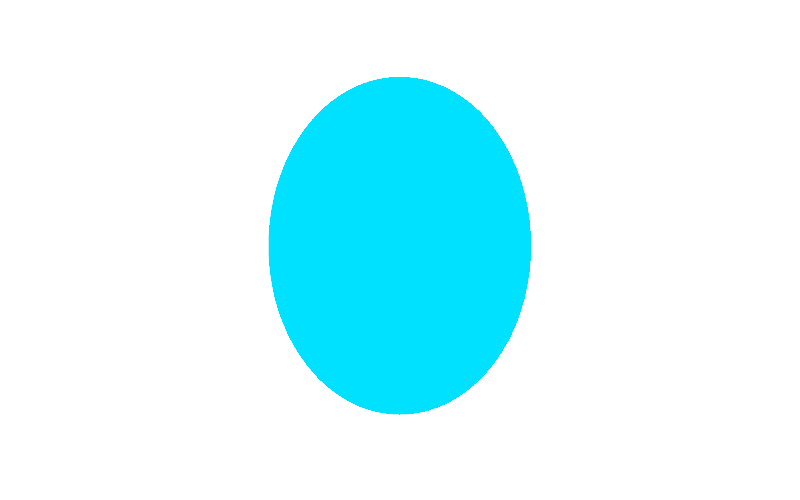
\includegraphics[height=1.5em]{figures/neurons/ica3.png}}}$ CA3 inhibitory}
  & $20 \pm 7$                              & \textcite{tukkerDistinct2013}
  & & \\
  & $17 \pm 7$                              & \textcite{laprayBehaviordependent2012}
  & & \\
  & $8.2 \pm 5.6$                           & \textcite{leaoOLM2012}
  & & \\
\bottomrule
\end{tabular}}
\caption{%
  \textit{In vivo} firing rates and population sparsity for each cell type.
  Values are mean $\pm$ SD\@. \textsuperscript{max} maximum observed rate.  $\approx$ approximate value read from figure.
}
\label{tab:firing_rates}
\end{table}
